\documentclass[border=10pt]{standalone}
\usepackage[svgnames]{xcolor}
\usepackage{amsmath}
\usepackage{pgfplots}
\pgfplotsset{compat=newest}
\usepackage[sfdefault]{FiraSans}
\usepackage{FiraMono}
\renewcommand*\familydefault{\sfdefault}
\begin{document}
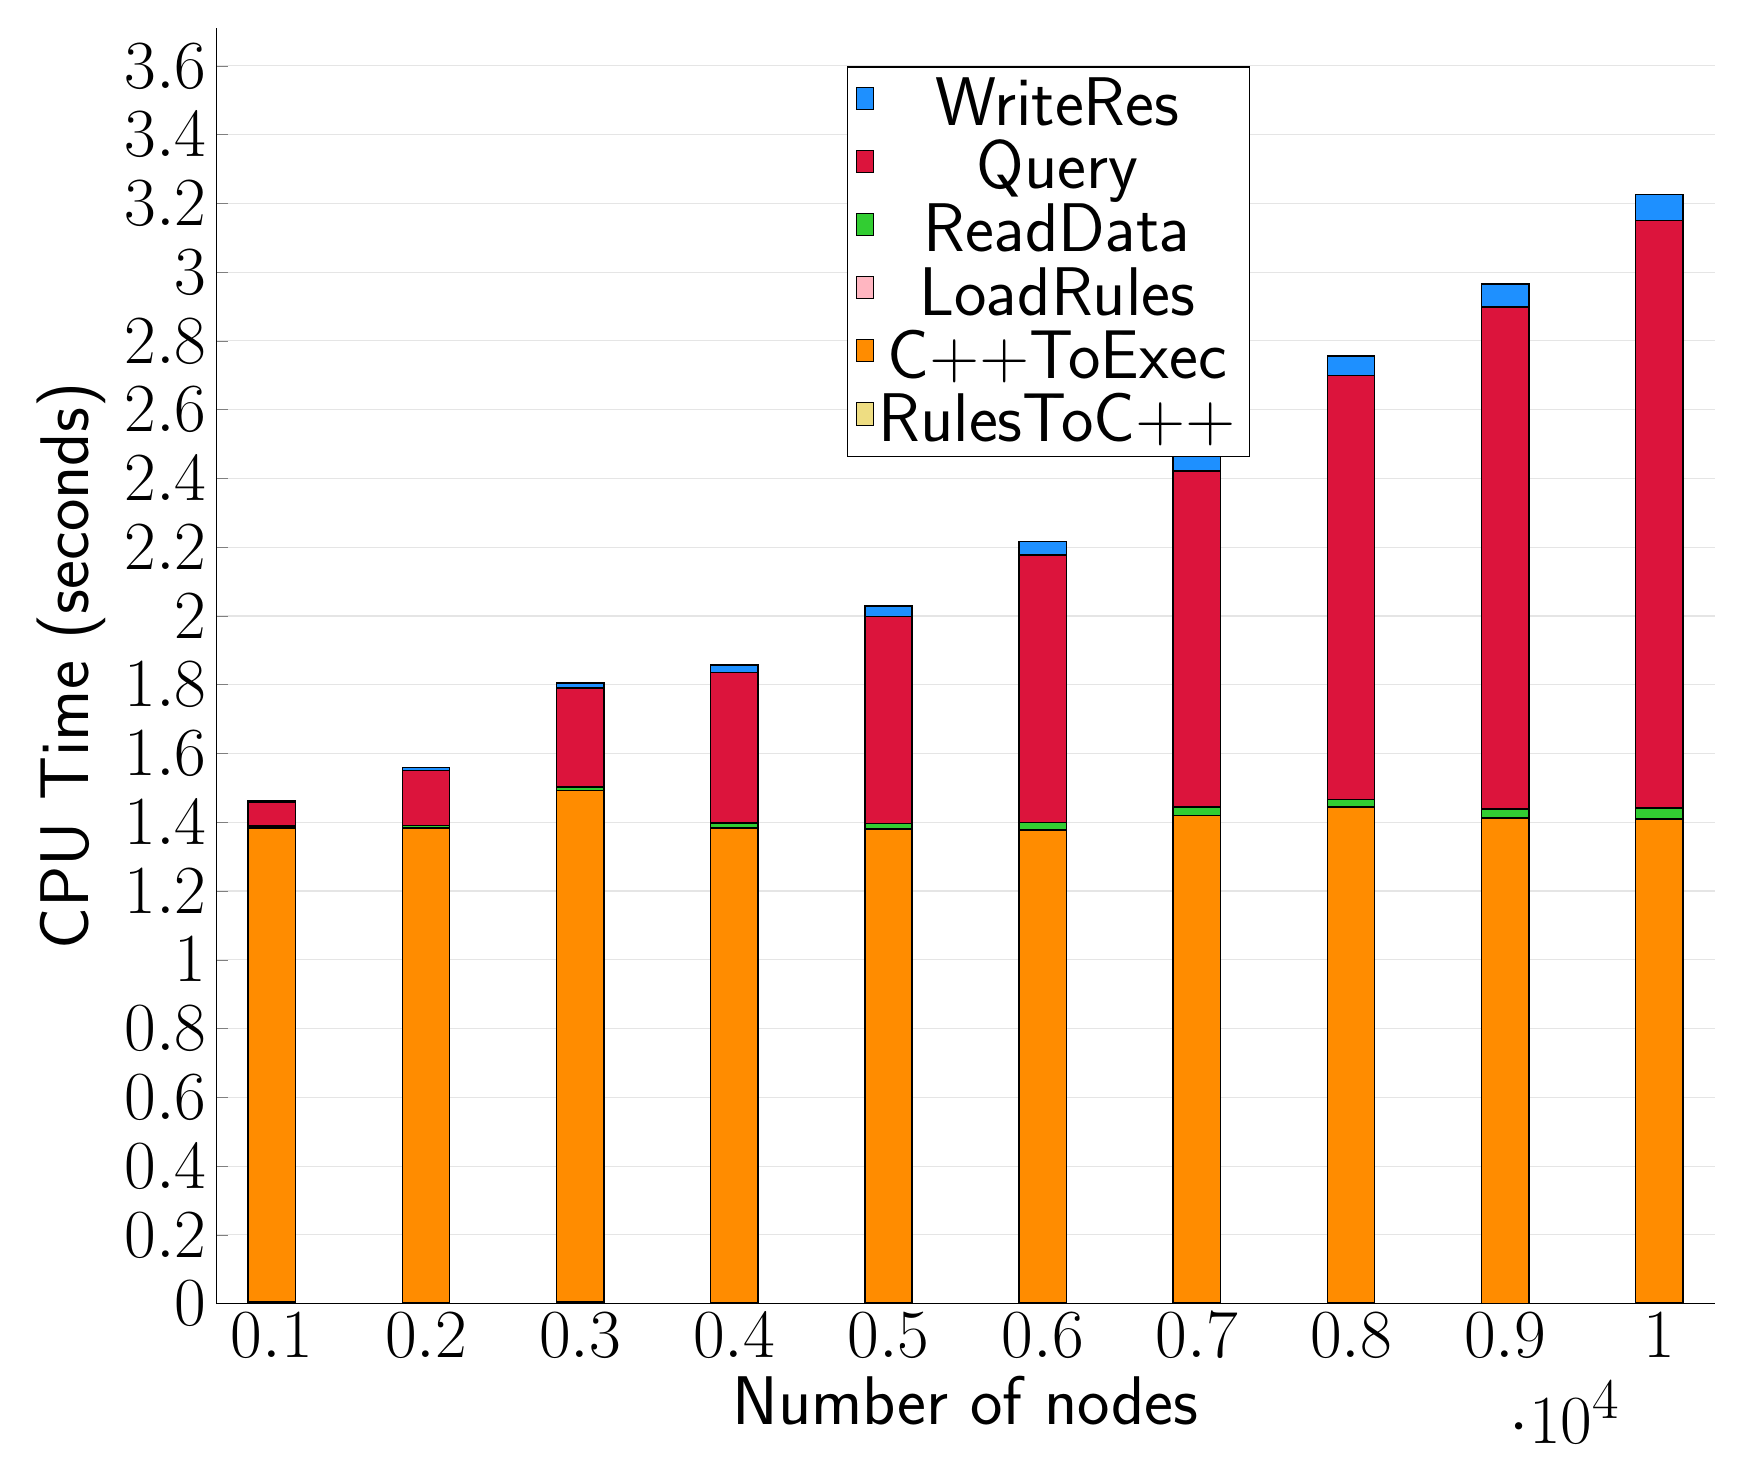
\begin{tikzpicture}
\begin{axis}[
   ybar stacked,
   width=1.7\textwidth,
   bar width=0.6cm,
   ymajorgrids, tick align=inside,
   major grid style={draw=gray!20},
   xtick=data,
   ymin=0, ymax=3.70944,
   axis x line*=bottom,
   axis y line*=left,
   enlarge x limits=0.04,
   legend style={
       at={(0.69, 0.97)},
       anchor=north east,
       legend columns=1,
       font=\Huge,
   },
   ylabel={CPU Time (seconds)},
   xlabel={Number of nodes},
   label style={font=\Huge},
   tick label style={font=\Huge},
]
\addlegendimage{fill=DodgerBlue, draw=black, line width=0.2pt}
\addlegendentry{WriteRes}
\addlegendimage{fill=Crimson, draw=black, line width=0.2pt}
\addlegendentry{Query}
\addlegendimage{fill=LimeGreen, draw=black, line width=0.2pt}
\addlegendentry{ReadData}
\addlegendimage{fill=LightPink, draw=black, line width=0.2pt}
\addlegendentry{LoadRules}
\addlegendimage{fill=DarkOrange, draw=black, line width=0.2pt}
\addlegendentry{C++ToExec}
\addlegendimage{fill=LightGoldenrod, draw=black, line width=0.2pt}
\addlegendentry{RulesToC++}
\addplot +[fill=LightGoldenrod, draw=black, line width=0.55pt] coordinates {
(1000, 0.004000000000000001)
(2000, 0.0020000000000000018)
(3000, 0.004000000000000001)
(4000, 0.001999999999999999)
(5000, 0.0020000000000000018)
(6000, 0.0020000000000000018)
(7000, 0.001999999999999999)
(8000, 0.001999999999999999)
(9000, 0.0)
(10000, 0.001999999999999999)
};
\addplot +[fill=DarkOrange, draw=black, line width=0.55pt] coordinates {
(1000, 1.3800000000000003)
(2000, 1.3820000000000001)
(3000, 1.4880000000000002)
(4000, 1.3820000000000001)
(5000, 1.3780000000000001)
(6000, 1.3760000000000001)
(7000, 1.418)
(8000, 1.4420000000000002)
(9000, 1.412)
(10000, 1.4080000000000001)
};
\addplot +[fill=LightPink, draw=black, line width=0.55pt] coordinates {
(1000, 0.0001596)
(2000, 9.779999999999999e-05)
(3000, 0.0001132)
(4000, 0.0001188)
(5000, 0.0001524)
(6000, 0.0001554)
(7000, 0.0001618)
(8000, 9.759999999999999e-05)
(9000, 0.00011640000000000001)
(10000, 0.0001494)
};
\addplot +[fill=LimeGreen, draw=black, line width=0.55pt] coordinates {
(1000, 0.004485599999999999)
(2000, 0.0066636)
(3000, 0.010914)
(4000, 0.013508800000000001)
(5000, 0.0169124)
(6000, 0.0210512)
(7000, 0.0237094)
(8000, 0.022048599999999998)
(9000, 0.0264422)
(10000, 0.0311866)
};
\addplot +[fill=Crimson, draw=black, line width=0.55pt] coordinates {
(1000, 0.0691302)
(2000, 0.1599118)
(3000, 0.2874434)
(4000, 0.43819539999999996)
(5000, 0.6014842)
(6000, 0.7787678)
(7000, 0.978196)
(8000, 1.233848)
(9000, 1.46015)
(10000, 1.70944)
};
\addplot +[fill=DodgerBlue, draw=black, line width=0.55pt] coordinates {
(1000, 0.0035027999999999995)
(2000, 0.008841)
(3000, 0.015191399999999999)
(4000, 0.022240799999999998)
(5000, 0.030053399999999997)
(6000, 0.0383444)
(7000, 0.0465276)
(8000, 0.056541799999999996)
(9000, 0.0665974)
(10000, 0.07548940000000001)
};
\end{axis}
\end{tikzpicture}

\end{document}
